\section{Basilisk a suited software to perform massive DNS calculations.}

In view of the previous research (especially the study of \citet{innocenti2020direct}) and the good results obtained in \citet{Naanouh2021numerical}, we thought that the partial differential equation solver, Basilisk (from \url{basilisk.fr}), was the most suited code to carry out tri-periodic simulation of buoyant droplets. 
Originally this code is based on the older code,  \texttt{Gerris}, and was developed primarily by Francesco De Vita, Jose-Maria Fullana, Geoffroy Kirstet-ter, Pierre-Yves Langrée, Emily Lane, Jose Lopez-Herrerra, John MacFarlane, Stéphane Popinet, Clément Robert, and Antoon van Hooft .
Both codes are open source, that is why since then the community contributed to the development of Basilisk and numerous authors published their contribution to the code in scientific reviews.
The open source aspect of Basilisk is somewhat essential for us since it enable us the to develop any desired features.
Besides, a lot of benchmarks demonstrated the good performances and the broad abilities of Basilisk.
All the algorithms are developed in C, if well done this language has the great advantage of optimizing the memory management, resulting in a better computation efficiency. 
Moreover, a lot of physical solvers are already implemented in the code, from wave modeling \citet{mostert2022high} to the simulation of suspended solid particles in a fluid using immersed boundary method \citet{shui2015direct}.
A last feature that has been recently implemented in Basilisk is the multilayer solvers \citep{popinet2020vertically} which will be of great interest in the modeling of film drainage problems. 
We refer the reader to this link \url{http://basilisk.fr/src/README} to see the whole range of possibilities offered by Basilisk.
Nevertheless, the most interesting feature for our use is the capability of modeling two phase flow in Basilisk. 
Indeed, the Volume-Of-Fluid (VOF) method implemented in Basilisk have shown great performance and accuracy, (see \citet{popinet2009accurate}\citet{popinet2018numerical}). 
This point will be developed in a following section since it is of major importance. 
Another practical aspect of Basilisk is that the meshing is included in the workflow of the simulation. 
This enables the possibility of switching between 2D cases and 3D cases automatically, indeed the \textit{dimension} parameter need to be switch from 2 to 3 the rest is automatic. 
In our case it is of a great use since we will start by carrying out 2D simulations and after validation we will switch to 3D mesh.
Speaking of the mesh, Basilisk provide several mesh types that considerably improve the efficiency of the calculation.
The first one is the classic Cartesian mesh, it is fully orthogonal, this is the most for mono-scale problem.
Another interesting grid is the adaptive mesh, as indicate by its name this mesh refines the area where high velocity gradients is observed.
\citet{innocenti2020direct} model a large quantity of bubbles in a container, this was only possible thanks to the adaptive mesh solver, otherwise it would have been too expansive.
The simulation of wave crashes by, \citet{mostert2022high} was made possible also thanks to the adaptive mesh refinement.
Numerous other examples testify of the usefulness of the adaptive mesh refinement solver.   
Then the last meshing technics is a subcase of the adaptive mesh, it is the \texttt{multigrid} mesh, presented in \citet{popinet2003gerris} for the incompressible Euler equations, and more recently in \citet{popinet2015quadtree} for the fully-nonlinear Boussinesq wave equations. 
This meshing technics consist in working with different levels of refined grids simultaneously.
More details will be given about the meshes in this section. 
Finally, the last point on which we would like to emphasize is that Basilisk is a self independent software (i;e. Only the source code of basilisk is needed to compile it) and simulations are launch via C files. 
Which makes it practical for the execution on any machines (cluster or not). 
In the next sections we present the specificity of the VOF methods, needs we speak more specifically about our numerical setup to model rising suspension of droplets. 



\subsection{The Volume Of Fluid Method}

The VOF method is used to model two-phase (or more) flows. 
The governing equations, solved by our solver in the present case, are the one-fluid formulation equation of momentum and mass, presented in \ref{chap:avg}. 
We recall their form here, 
\begin{equation}
    \pddt (\rho \textbf{u})
    = \nablabh \cdot (\textbf{T} -\rho  \textbf{u} \textbf{u})
    + \textbf{b}
    + \textbf{f}_I\delta_I
    \;\;\;\text{and}\;\;\;
    \pddt \rho
    = 
    - \nablabh\cdot(\rho\textbf{u}_k). 
\end{equation}
Note that the material properties (i.e. $\rho$ and $\mu$) takes the value of the phase in presence. 
As seen in \ref{chap:avg}, in two phases flows we define a phase indicator function $\chi$, which is a marker to identify the phases in presence.
When, $\chi = 1$, we are located in the dispersed phase, when $\chi = 0$ in the fluid phase for example, therefore $\chi$ correspond to a Heaviside function. 
However, the Heaviside function is not continuous and derivable everywhere. 
This latter point makes the use of $\chi$ impossible in numerical method.
Therefore, in CFD code, we use an approximation of the Heaviside function, namely the color function $C$. 
Since we want to follow the phases with time,  we need to add the equation of transport of $C$ to complete the system, namely,
\begin{equation}
    \frac{\partial C}{\partial t} + \textbf{u}\cdot\bm{\nabla} C = 0.
    \label{eq:cfunc} 
\end{equation}
At this point several methods are available to define $C$ and to discretize these equations. 

Regardless of the definition of $C$ it is important to say a few words on the discretization of the Navier-Sokes equations which is independent of this choice. 
Basilisk uses the finite volume based method to discretize the governing partial differential equations.
A full review of the finite volume method is made in the book \citet{ferziger2002computational}.
The finite volume method consists in discretizing the whole domain of fluid by finite volume called cells. 
This discretized domain is what we call a mesh. 
In Basilisk we use only orthogonal meshes. 
Which means that the cells of the domain are only squares or cubes.
Nevertheless, as mentioned in introduction there are several specificities among these orthogonal grids.   
\begin{figure}[h!]
    \centering
    \begin{tikzpicture}
        \node (a) at (-0.25\textwidth,0){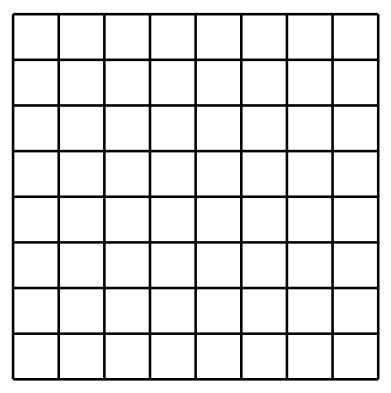
\includegraphics[height = 0.2575\textwidth]{image/pic/Uniforme.png}};
        \node (b) at (0,0){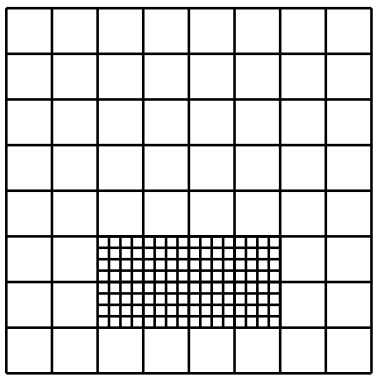
\includegraphics[height = 0.25\textwidth]{image/pic/non-uniform.png}};
        \node (c) at (0.25\textwidth,0){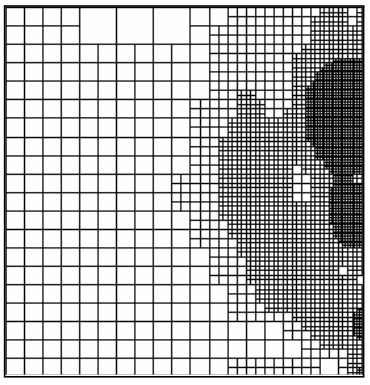
\includegraphics[height = 0.25\textwidth]{image/pic/adaptativemesh.png}};
        \node (leg) at (a.south){(a)}; 
        \node (leg) at (b.south){(b)}; 
        \node (leg) at (c.south){(c)}; 
    \end{tikzpicture}
    \caption{Different type of orthogonal meshes. (a) uniform mesh, (b) Non-uniform mesh, (c) Adaptive \textit{Quad/Octree} mesh. Reprinted from \citet{mani2021numerical}. }
    \label{fig:meshes}
\end{figure}
The first one is the classic uniform grid depicted \ref{fig:meshes} where all the cells have the same size.
The second one is the non-uniform grid. 
It is useful when the user need to refine a specific area of the mesh, due to high local gradient of the velocity for example.
Then, the last one, is the Adaptive \textit{Quad/Octree} Grids, on which we are to give a bit more details.
It consists in subdividing the cells into $2^2$ cells in two dimension, or in $2^3$ cells in 3 dimension. 
Each cell that have the same size form a group.
All the groups are referred by their respective \textit{levels}. 
The group of level 0 is the one with the larger cells size, actually at this there is only one cell of the size of the domain. 
Then as we look at higher levels the size of the cells decrease. 
Besides, Basilisk offer the possibility of the \textit{Adaptive} option. 
Which means that the cells are subdividing or merging themselves automatically all along the simulation time. 
At the frontier between two levels there is what we called the \textit{resolution boundary}. 
Those boundaries, are somewhat problematic since the cells on each side are not of the same size.
Therefore, the basic operation of the finite volume method are not trivial anymore. 
To avoid this issue Basilisk use \textit{halo cells}.
One \textit{halo cell} is the representation of the cell of the lower level that gather the mean value of the four smaller cells.
The former cell is of the same size of the cell at the other side of the \textit{resolution boundary}, that is why the system is consistent. 
In Basilisk the cells from which the \textit{halo cells} are build are called the children cells, therefore the lower level cells are the parent cells. 
This principle is used for the adaptive mesh, nevertheless, the \textit{Quad/Octree} grid has one subclass, the \textit{multigrid} mesh. 
This meshing technics is no more than a uniform mesh where we make use of the \textit{halo cells}, and parent/children principle. 
Even though there is no \textit{resolution boundary}, this technics allows the user to loop through different levels and through each branch of the mesh. 
This feature is of a great interest to carry out fast operations on vector or scalar fields. 
We refer to the publication of \citet{popinet2015quadtree} for a more detailed explanation.  
Once the mesh is set one need to discretize the governing equations in space and time (see \citet[chapter 3]{tryggvason2011direct}). 

Five main option exist to define the color function $C$ :
the volume of fluid method,
the front taking method,
the level-set method,
the phase-field method
and the CIP method.
As the title of this section is the \textit{volume of fluid method} one could guess which one we use. 
For more details on the other methods we refer the reader to \cite[Chapter 4]{tryggvason2011direct}. 
With the Volume-of-fluid method the color function is now defined by a \textit{VOF tracer}, $f_i$, where $k$ stand for the indices referring to the phase. 
For $N$ VOF tracer $f_k$ is defined for $0\leq k\leq N$.
From $k=0$ for the continuous phase to $k=1$ to $N$ for the dispersed phases (in case we have $N$ dispersed phases). 
In practice the function $f_c$ is not computed since we have the relation, $f_c = 1- \sum_{k=1}^N f_k$. 
The value of the $f_k$ is comprised between $0$ and $1$.
$f_k = 0$ meaning that the concentration of phase $k$ is null, $f_k = 1$ meaning that $100\%$ of the volume is occupied by the phase $k$. 
Note that in every cell the value of $f_k$ is either $0$ or $1$, except in the cells including an interface where the value is the percentage of the phases in presence.
\begin{equation}
    f_k = \left\{\begin{tabular}{cc}
        $1$  &if $\textbf{y}\in V_k$\\
        $0$  &if $\textbf{y}\in V_c$\\
        $0$ to $1$  &if $\textbf{y}\in V_c \cap V_k$\\
    \end{tabular}
    \right.,
\end{equation}
where $V_k$ is the volume occupied by the phase $k$.
The overall condition is that $\sum_k^N f_k \leq 1$.
Next, if we note $\rho_k$ and $\mu_k$ the material property of phase $k$ we can finally compute in each cell the value of the material properties,
\begin{equation*}
    \rho 
    = \sum_k^N \rho_k f_k 
    + (1-\sum_k^Nf_k)\rho_c 
    \;\;\;\text{and}\;\;\;
    \mu 
    = \sum_k^N\mu_k f_k 
    + (1-\sum_k^Nf_k)\mu_c.
\end{equation*} 
In the neighboring cells of the interfaces the calculation of $\rho$ and $\mu$ are slightly different \citep{tryggvason2011direct}. 
Then, once the material properties are calculated, the Navier-Stokes equations solved and the VOF tracers advected, the last step is to reconstruct the interfaces from the $f_k$.
To do so, several methods, more or less accurate, are available  to us.
\ref{fig:VOF} depicts the different reconstruction method, namely, the Simple Line Interface Calculation or SLIC method, the Hirt and Nichols reconstruction method and the Piecewise Linear Interface Calculation or PLIC method. 
As we can clearly see on the scheme the methods goes from coarse (with SLIC) definition of the interface to a more accurate reconstruction (with PLIC).
\begin{figure}
    \centering
    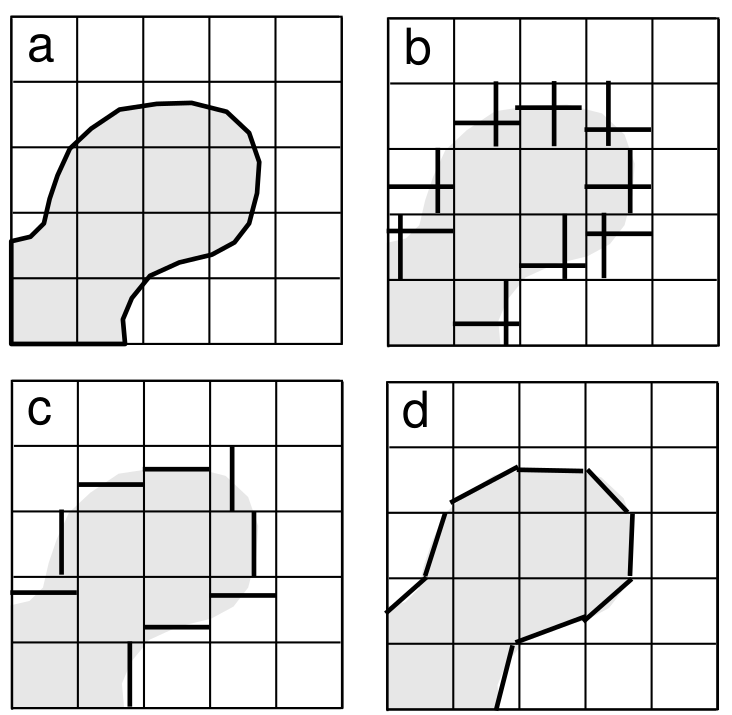
\includegraphics[width = 0.4\textwidth]{image/pic/VOF.png}
    \caption{VOF reconstruction of the solution for advection in two dimensions. 
    (a) The original interface. 
    (b) The original SLIC reconstruction. 
    (c) The Hirt and Nichols reconstruction. 
    (d) PLIC reconstruction. 
    Reprinted from \citet{tryggvason2011direct}.}
    \label{fig:VOF}
\end{figure}
In Basilisk we use PLIC method using height functions (see \citet[Chapter 5]{tryggvason2011direct}). 
Here is a quick summary of how height functions work.
Each segment is parametrized by its normal $\textbf{n}$ and the intercept of a line, $\alpha$. 
Then, in the local reference frame of coordinate $\textbf{z}$, it is possible to define the interface by,
\begin{equation}
    \textbf{n}\cdot\textbf{z} 
    = \alpha,
\end{equation}
where $\alpha$ is computed with the local volume fraction of the phase and the unit normal. 
The overall error is of second order. 
Nevertheless, it must be said that even though the PLIC method is accurate, it still has some draw back sheared with the two other methods. 
Indeed, if we consider 2 tracers the interface is reconstructed considering the tracer $f_c$ and the tracer $f_1$.
Which is equivalent to consider two phases, up to now everything is normal. 
But, consider two interfaces getting closer, then at some point the interfaces will merge together discarding the physical aspect.
Indeed, since we compute height functions from the local volume fraction, if two drops with the same tracer met, then the interfaces are reconstructed regardless of the physical geometry. 
Another problem is that VOF tracers are advected separately so interpenetration of different VOF tracers can happen (this issue will be developed in the next section). 
These two facts mandate the use of a relatively fine mesh so that the film between the droplets is partially resolved.

Once the interface is reconstructed, we can tackle the most challenging problem of VOF simulations.
Which is the modeling of the surface tension forces, i.e. the source term, $\textbf{f}_I\delta_I$, in the one-fluid formulation equations.
Obviously we will not detail the solutions here, to get an overall vision of the problem we refer the reader to \citet{popinet2018numerical} or  \citet[Chapter 7]{tryggvason2011direct}.
However, we can cite the two most basic method.
The first one is the \textit{Continuous surface force method}, in consist in discretizing the expression of the surface force source term. 
Note that the expression of $\delta_S$ make use of the color function, it is in fact equal to the gradient of the color function. 
The approximation of the surface force source term is then,
\begin{equation}
    \sigma \kappa  \textbf{n} \delta_I 
    = \sigma \kappa \nabla f_i,
\end{equation}
where the curvature $\kappa$ is estimated through height function \citep{popinet2018numerical}. 
The other method is the \textit{Continuous surface stress method} which is equivalent, but instead of discretizing the force term, we discretize the divergence of a stress.
It reads, 
\begin{equation}
    \textbf{f}_I \delta_I = \nabla \cdot \left[\sigma (\textbf{I}-\textbf{nn})\delta_I\right],
\end{equation}
\tb{Find were does that came from}
which is valid even with non-constant $\sigma$. 
In Basilisk, we make use of the former method. 

The overall difficulty encountered in the two-phase flows simulations is to manage the singularities at the interfaces.
Indeed, it is a common problem in mathematic when the function is not derivable everywhere.
Hence, from a numerical point of view it is no less of a problem. 
In the conclusion of this chapter we will review some issues arising in  the simulation of emulsion because of this point. 

\subsection{Numerical coalescence}

As briefly mentioned in the preceding section, numerical coalescence can occur during a simulation if two interfaces are one cell mesh apart (assuming there is a solely VOF tracer). 
However, in \ref{chap:avg} we showed that the coalescence of two droplets is a multiscale phenomenon. 
At first, it involves hydrodynamical and lubrication forces.
Once the interfaces are close enough Van deer Waals forces are responsible for the coalescence.
The former forces are well modeled when using a fine enough mesh. 
Indeed, we solve the Navier-Stokes equation together with the transport of the color function, which is the basis of the calculation of the lubrication forces \citep{guazzelli2011}. 
However, the latter contribution involve microscale interaction which are not included in this model.
Even though, it is possible to include Van der Waals forces in Basilisk, it would be too expensive to compute the film drainage problem for several droplets at the same time.
To avoid this problem \citet{thomas2010multiscale} modeled the film drainage by allowing coalescence when the contact time of the droplet is greater than the critical time of contact (computed theoretically).  
However, the closure for the contact time is not well define for our parameters yet.
Moreover, before allowing coalescence after a critical time, we need to prevent it anyway. 
Hence, in any cases we need to prevent coalescence event to happen since DNS of the film drainage is too expansive numerically. 
Besides, to create accurate closures terms seen in \ref{chap:avg}, we need to identify accurately the topology of a given situation.
This way we will be able to give the value of a closure term in terms of the exact number and size of the droplets for example. 
This implies that we must keep a constant number of droplets all along the simulation.

Before avoiding coalescence to happen it is important to identify why it does happen. 
The reason why numerical coalescence occurs is that only one VOF tracer is used. 
Indeed, let's take two drops approaching each other. 
The VOF tracer is advected along the velocity fields. 
We recall that in the interfacial area the VOF tracer has a transitional value between $1$ and $0$. 
Therefore, when the drops eventually get close enough the VOF tracer at the interface of the drops meet each other in the same cells. 
Since the same VOF tracer is used for the two droplet, it results in the addition of the values of the VOF tracer at the interfaces since they gather in the same cells. 
Then, as the VOF tracer merge it is impossible to reconstruct the interface of the respective droplets. 

Using different VOF tracer would prevent the drops to coalesce 
Indeed, during advection the VOF tracer will not sum with the neighboring ones thus the reconstruction of the interface will be possible. 
However, in the literature, we see that we need about hundreds of particles to be able to get a representative volume. 
And since we need to advect each VOF tracers independently, it would be too expensive to have one VOF tracer per drops.    
Luckily, we only need that the adjacent droplets at a given time $t$ have different VOF tracer. 
In 2D the famous \textit{four color map theorems} stipulate that we only need 4 color to color adjacent country with a different color (this is a topological proof).
For our concern, it does mean that we will need no more than four VOF tracer in order for the adjacent droplets to have different VOF tracer. 
In 3D this theorem is not valid anymore. 
Moreover, the droplets move within time thus their neighboring particles changes, and they might need a different VOF tracer.

To tackle this issue \citet{mani2021numerical}, developed an algorithm on Basilisk to carry out the previous task automatically. 
Even though, this algorithm is based on empirical observation and not topological arguments it prevents from using too much VOF tracer. 
The workflow is as follows.
In a first step we identify the VOF tracer having droplets that are close to each other. 
Then for each of these VOF tracers, we identify the pairs of droplets. 
Then we check which of the droplets among one pair have the least neighbors. 
Finally, we switch the VOF tracer of the former droplet to a new tracer that is not in the vicinity of the droplet. 
If no VOF tracer is available then we create a new one. 
In the practical case we indeed notice that 2D simulations do not use more than 4 VOF tracers. 
Therefore, this is a proof of the efficiency of the algorithm. 
This algorithm considers a droplet close to another one only if they have VOF tracers two cells apart.
Consequently, if the drops relative velocity is greater than that this length time the time step then the algorithm will not work.
Nevertheless, in practice the CFL condition is respected which means that the distance traveled by a fluid particle is never superior to one mesh cell. 
This algorithm is launched every time step by default, nevertheless we could call it every 2 time steps (since three would be a bit reckless). 


\tb{more details on this matter }
\subsection{Simulation of periodic rising droplets}
As concluded in the two previous sections, we are going to make DNS of a random array of droplet rising in a continuous Newtonian fluid with the code Basilisk. 
Therefore, in this section we are going to present the 


In Basilisk the computational domain of the simulation must be a square in 2D or a cube in 3D, as depicted on \ref{fig:numscheme}. 
Depending on the desired number of bubbles $N_b$ we divide the domain of size $\mathcal{L}$ in $N$ smaller squares of length $\Delta$.
In each smaller squares we initialize the VOF tracers $f_i$ as a spherical, in 3D, or circular, in 2D, shaped area representing the droplets.
Each droplet of diameter $L$ is centered inside their $\Delta\times \Delta$ square.
Besides, we add a random shift vector for each droplet position so that all the simulations with the same parameters are unique. 
The shift must be limited in order to avoid that the drops touch each other at the initialization time (in which case they would immediately merge).   
Also, another method consist of initializing all droplets randomly, making sure that they are initially far enough so that they do not touch each other at the first step of the simulation.
The latter technics was used in the simulation performed in \ref{chap:mono-disperse} since it has shown faster convergence. 
Indeed, as we initialize with a random state, the suspension takes a shorter amount of time to reach it statistically random steady state. 
\begin{figure}[h!]
    \centering
    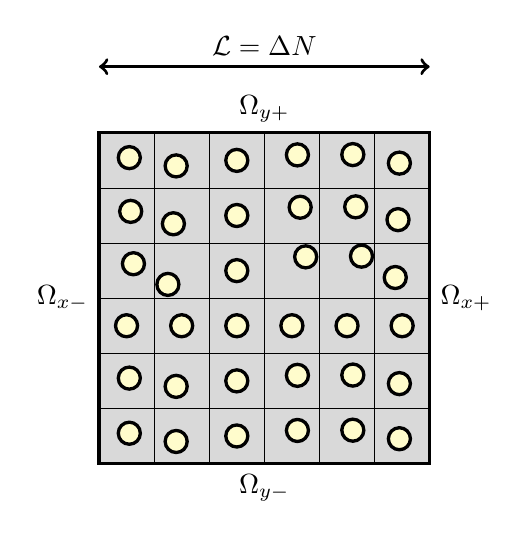
\begin{tikzpicture}[very thick,scale = 0.7]
        \draw[fill=gray!30](0,0) rectangle(6,6);
        \foreach \x/\dx in {0.5/0.1,1.5/-0.2,2.5/0,3.5/0.2,4.5/0.21,5.5/-0.1}{
            \draw[very thin](\x+0.5,0)--(\x+0.5,6);
            \draw[very thin](0,\x+0.5)--(6,\x+0.5);
            \foreach \y/\dy in {0.5/0.1,1.5/+0.1,2.5/0,3.5/0.25,4.5/0.15,5.5/0.1}{
                \draw[fill=yellow!20](\x+\dx*\dy*5,\y+\dy*\dx*5) ellipse(0.2 cm and 0.2 cm);
            }
        }
        \draw[<->](0,7.2)--(6,7.2)node[midway, above]{$\mathcal{L} = \Delta N$};
        \draw(3,6)node[above]{$\Omega_{y+}$};
        \draw(3,0)node[below]{$\Omega_{y-}$};
        \draw(6,3)node[right]{$\Omega_{x+}$};
        \draw(0,3)node[left]{$\Omega_{x-}$};
    \end{tikzpicture}
    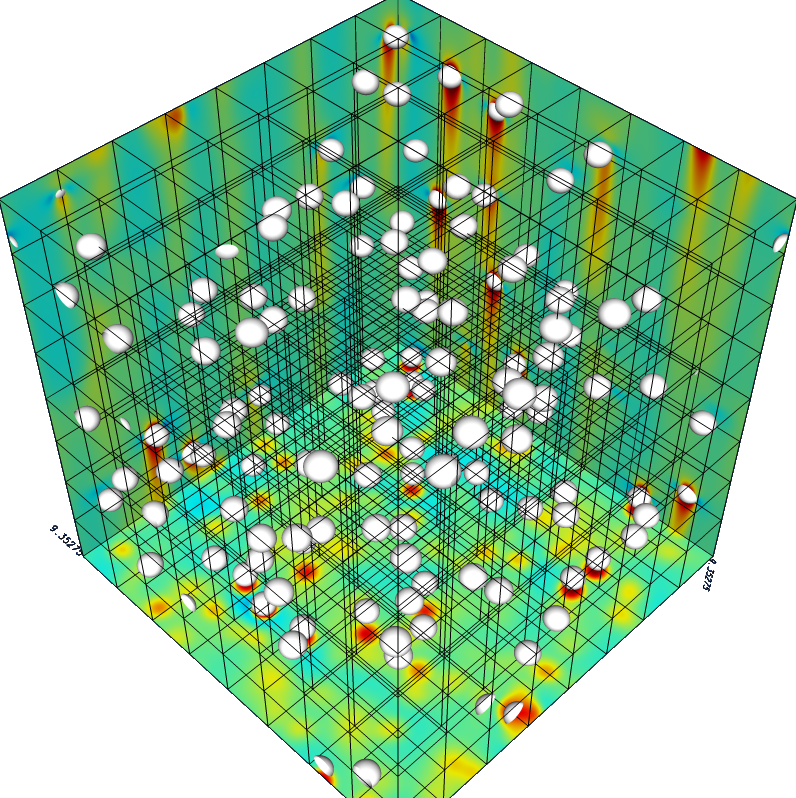
\includegraphics[width=0.45\textwidth]{image/3D/PHI01.png}
    \caption{(left) Scheme of the initialization of an array of droplets immersed in a 2D periodic domain.
    (right) Picture of a 3D simulation with $\phi = 0.1$, $N = 5$ the color represent the velocity field.}
    \label{fig:numscheme}
\end{figure}

The dimensionless parameters of this study have been already discussed in \ref{chap:avg}.
Nevertheless, additional dimensionless parameters must be introduced since numerical parameters that weren't on the theoretical problem appear. 
Only six parameters are needed among the existing dimensionless parameters. 
However, the numerical simulations involve an others length parameters among the ones already mentioned in \ref{sec:introavg}, namely the length of a cell in the mesh.
Therefore, we need to define a new dimensionless parameter, namely, the number of cells per diameter refer by $\delta$. 
From those parameters it is possible to recover the physical parameters needed by the simulation. 
But before we fix the following parameters, $\rho_d = L = g = 1$ for convenience.
Then it yields the following relations to recover the remaining parameters,
\begin{align*}
    &\rho_c = \rho_d\rho_r ,&
    &\mu_d  =\frac{\rho_d \sqrt{|1-\rho_r| \rho_r g \bar{L}^3}}{\mu_r Ga},&
    &\mu_c  = \mu_d\mu_r,&
    &\delta  = D/Nc& \\
    &\sigma = \frac{|1-\rho_r|\rho_d g L^2}{Bo},&
    &\Delta = \sqrt{\frac{\pi D^2}{4\phi}},&
    &\mathcal{L} = \Delta \sqrt{N_b}.&
\end{align*}
From those parameters it is possible to define different time, length and velocity scales. 
It will be useful when we will need to make the results dimensionless. 
The different scales in which we will be interested in are the following.
\begin{align*}
    &U_\mu = \frac{g D^2 \Delta \rho}{\mu_c}&
    &U_\rho = \sqrt{\Delta \rho \frac{Dg}{\rho_d}}&
    &U_\sigma = \sqrt{\Delta \rho \frac{Dg}{\rho_d}}& \\
    &T_\mu = \frac{\mu_c}{g\Delta \rho D}&
    &T_\rho = \sqrt{\frac{\rho_dD}{g\Delta\rho}}&
    &T_\sigma = \sqrt{\frac{\rho_{avg} D^3}{\pi \sigma}}&
\end{align*}
Were $U_\mu$, $U_\rho$ and $U_\sigma$ are respectively the viscous inertial and capillary velocity scales. 
Similarly, $T_\mu$, $T_\rho$ and $T_\sigma$ are the corresponding time scales. 
Here is a quick explanation of the physical meaning of those scales :
When $Ga \ll 1$, in one unit of $T_\mu$ a droplet travel a distance of $D$ relatively to the fluid.  
Similarly, When $Ga \gg 1$ a droplet travel a distance of $D$ in one unit of $T_\rho$. 
Lastly, the Capillary time $T_\sigma$ will be the period of one undulation of the surface droplet. 
Of course this scale provide us with an order of magnitude, they aren't exact. 

In Basilisk the set-up of a simulation (solvers and parameters) is made by including or excluding header files.
All the header files can of course be found in the sources of the code (\url{http://basilisk.fr/src/}).   
In the following, we describe the header files used in this simulation. 
The first one has in fact already been mentioned, it is \href{http://basilisk.fr/src/grid/multigrid.h}{multigrid.h} or  \href{http://basilisk.fr/src/grid/multigrid3D.h}{multigrid3D.h} file for 3D simulations. 
It set up a uniform staggered multigrid mesh. 
Then, we add the file \href{http://basilisk.fr/src/navier-stokes/centered.h}{centered.h} to resolve Navier Stokes equation on this mesh with centered formulation.
The \texttt{two-phase.h} header set up the VOF tracers and interfaces for two immiscible fluid.
It also set add transport equation of the VOF tracers coupled with the Navier Stokes solver.
To account for the tension surface forces mentioned in the previous section we include the \href{http://basilisk.fr/src/tension.h}{tension.h} header file. 
This file takes in account the curvature calculation of the interface and the interfacial forces. 
We then add the \href{http://basilisk.fr/sandbox/fintzin/Rising-Suspension/no-coalescence.h}{no-coalescence.h} header which create several VOF tracers depending on the needs in order to avoid coalescence. 
Finally, the \href{http://basilisk.fr/src/view.h}{view.h} and \href{http://basilisk.fr/src/output.h}{output.h} header are included manage the graphical output.  

As mentioned earlier  the boundaries of the domain are periodic. 
It signifies that the velocity field follow the these conditions,
\begin{align}
    \bm{u}(y_i = 0,t) = \bm{u}(y_i = \mathcal{L},t) \;\;\; &\forall \bm{y} \in \Omega_{y_i-} \;\;\;\text{and}\;\;\; \forall i \in \left\{1,2,3\right\}.\\
    \bm{u}(y_i = \mathcal{L},t) = \bm{u}(y_i = 0,t) \;\;\; & \forall \bm{y} \in \Omega_{y_i+} \;\;\;\text{and}\;\;\; \forall i \in \left\{1,2,3\right\}.
\end{align}
And the pressure fields respect similar conditions, 
\begin{align}
    p(y_i = 0,t) = p(y_i = \mathcal{L},t) \;\;\; &\forall \bm{y} \in \Omega_{y_i-} \;\;\;\text{and}\;\;\; \forall i \in \left\{1,2,3\right\}.\\
    p(y_i = \mathcal{L},t) = p(y_i = 0,t) \;\;\; & \forall \bm{y} \in \Omega_{y_i+} \;\;\;\text{and}\;\;\; \forall i \in \left\{1,2,3\right\}.
\end{align}
The advantage of using periodic domain is that we can run the simulations for an arbitrary long times since the droplets loop inside the domain.
Besides, it lets the flow develop freely, which is more physical for representative volume. 
However, it has some drawback.
The first  one is that the physical phenomenons that have a wavelength larger than the domain won't be represented. 
Therefore, the domain still needs to be large enough to represent the desired phenomenons.
And the other one is that, if we were to model the problem as it is, we would see both phases falling though a Cartesian multigrid mesh. 
Indeed, we apply an acceleration $g$ on the whole domain. 
And since our domain is periodic the velocity field will keep accelerating through the infinite domain.
If we discard the numerical issues this is not a problem.
Indeed, we could still measure the relative velocities and fluctuation over the domain. 
But, the thing is that we can not discard the numerical issues. 
Therefore, we set the simulation in the referential of the fluid phase by applying an acceleration $\bm{a}$ on the whole domain equivalent to a null averaged force.
Namely, 
\begin{equation}
    \textbf{a} = - \left[1-\frac{\left<\rho\right>}{\rho}\right]\textbf{g},
\end{equation}
where we use the volume average operator defined in \ref{chap:avg}.
We can notice that the contribution of the force on the whole numerical domain is null.
Indeed, it yields, 
\begin{equation}
   \int \rho\textbf{a} g(\textbf{x,y}) dV 
    = \textbf{g}\int \rho g(\textbf{x,y}) dV -\textbf{g}\left<\rho\right>\int g(\textbf{x,y}) dV 
    =0,
\end{equation}
where we recognized in the last equation the volume average of the density $\rho$.
Now, the net averaged velocity of the domain will be in null in both direction.
Besides, by applying a constant acceleration through the domain we preserved the relative motion.
However, it turns out that this last fact ins't true in practice. 
Indeed, numerical error accumulation of the momentum at the interfaces occurs due to the inconsistency of the numerical schemes (see \citet{popinet2018numerical}).
Besides, due to the discontinuity at the interfaces solvers can either conserve the momentum or the velocity depending on the numerical schemes used.
In our case we conserve the velocity and not the momentum. 
In Basilisk C we could use the \href{http://basilisk.fr/src/navier-stokes/conserving.h}{conserving.h} solver.
Anyhow, as this problem come from different source it is rather difficult to solve it properly.
As an example in the CFD-DEM code \href{https://hal.archives-ouvertes.fr/hal-02170320}{PeliGRIFF}
they directly force a null velocity fields inside the solver steps. 
As this solution is rather sophisticated we choose for another option. 
Indeed, to solve this problem we add an artificial acceleration on the whole domain at each time step. 
If $U_\epsilon$ is the bulk velocity (which should be theoretically null), then the acceleration to cancel this velocity must be equal to $U_\epsilon/\Delta t$ where $\Delta t$ is the current time step. 
In the next pages we will refer this artificial acceleration as the \textit{momentum correction}. 

